\documentclass{article}

\usepackage{arxiv}
\usepackage{amsmath}
\usepackage[utf8]{inputenc} % allow utf-8 input
\usepackage[T1]{fontenc}    % use 8-bit T1 fonts
\usepackage{hyperref}       % hyperlinks
\usepackage{url}            % simple URL typesetting
\usepackage{booktabs}       % professional-quality tables
\usepackage{amsfonts}       % blackboard math symbols
\usepackage{nicefrac}       % compact symbols for 1/2, etc.
\usepackage{microtype}      % microtypography
\usepackage{multirow} 
\usepackage{cleveref}       % smart cross-referencing
\usepackage{listings}
\usepackage{graphicx}
\usepackage{natbib}
\usepackage{doi}
\usepackage{float}
\usepackage{enumitem}


\title{Rapport préliminaire}

% Here you can change the date presented in the paper title
%\date{September 9, 1985}
% Or remove it
%\date{}

\newif\ifuniqueAffiliation
% Comment to use multiple affiliations variant of author block 
\uniqueAffiliationtrue

\author{\hspace{1mm}Alexandre Eberhardt\\
	Master of Computer Science\\
	Laval University\\
	Québec, QC \\
	\texttt{alexandre.eberhardt.1@ulaval.ca} \\
	%% examples of more authors
	\And
    \hspace{1mm}Rémi Hercouët \\
	Master of Computer Science\\
	  Laval University\\
	Québec, QC \\
	\texttt{remi.hercouet.1@ulaval.ca} \\
}

% Uncomment to override  the `A preprint' in the header
\renewcommand{\headeright}{}
\renewcommand{\undertitle}{}
\renewcommand{\shorttitle}{Rapport Préliminaire - IFT-7201}

%%% Add PDF metadata to help others organize their library
%%% Once the PDF is generated, you can check the metadata with
%%% $ pdfinfo template.pdf
\hypersetup{
pdftitle={Rapport préliminaire},
pdfsubject={q-bio.NC, q-bio.QM},
pdfauthor={Alexandre Eberhardt, Rémi Hercouët},
}

\begin{document}
\maketitle
\vspace{-0.5cm}

\begin{center}
    Code source du projet : \url{https://github.com/alexandreeberhardt/RL-FrozenLake}
\end{center}
\section{Cas d'étude}



\subsection{Description de l'environnement}
L'environnement \href{https://gymnasium.farama.org/environments/toy_text/frozen_lake/}{Frozen-lake} de la bibliothèque d'OpenAI \href{https://gymnasium.farama.org/index.html}{Gymnasium} possède plusieurs variables sur lesquelles il est possible d'influencer pour compléxifier et manipuler l'environnement considéré.

La première étant la \textbf{disposition de la carte} entièrement personnalisable en passant une matrice lors de la création de l'environnement. Les tuiles possibles sont :
\begin{itemize}
    \item F : Pour une tuile glacée où le déplacement est stochastique (Frozen);
    \item S : Pour la tuile de départ (Start):
    \item H : Pour une tuile terminale mais non ojectif (Hole);
    \item G : Pour une tuile terminale objectif (Goal). 
\end{itemize}
Ainsi le nombre de situations dangereuses (tuile H) et leur positionnement est entièrement personnalisable.

La seconde est la \textbf{probabilité de se déplacer} sur les tuiles F. En effet, comme on ne s'intéresse pas à des déplacements déterministes mais stochastiques, on peut spécifier la probabilité de succés de déplacement dans la direction souhaitée.

Enfin il est possible de choisir \textbf{la distribution des récompenses}. Notamment, on peut associer à chaque tuile une récompense lors que l'on arrive dessus, à l'exception bien sûr de la tuile de départ.

La \textbf{difficulté} de l'environnement va donc découler du \textbf{placement} et le \textbf{nombre de tuiles} Hole mais aussi la \textbf{probabilité de déplacement} sur les tuiles Frozen. On peut aussi \textbf{contraindre} l'agent à faire des choix plutôt que d'autres sur une même carte en modifiant les \textbf{récompenses}.
\subsection{Nos cas d'études}
La génération de chaque cas d'étude suit le code suivant :
\begin{lstlisting}[language=Python]
gym.make('FrozenLake-v1',
        desc=<matrice carte>,
        is_slippery=True, # active le deplacement stochastique
        success_rate= <proba deplacement>,
        reward_schedule=<rewards>,
        )
\end{lstlisting}
où \textit{<matrice carte>} est un tableau (array) de taille H composé de chaînes de caractères de taille W respectant les identifiants des tuiles (S, F, H et G), \textit{<proba deplacement>} est un nombre flottant représentant la probabilité de succès liée à un déplacement, et enfin \textit{<rewards>} représente la distribution des récompenses selon l'état d'arrivée.

Pour nos experiences, nous avons conçu trois cas d'étude distincts. Chacun isole et teste une composante spécifique du comportement de l'agent face à des niveaux de difficulté et des défis variés.

\subsubsection{Cas 1 : Efficacité pure}

\textbf{Description et défi :} Cette carte présente une grille assez vide avec quelques trous. Le but principal n'est pas la survie, mais l'optimisation. L'objectif est d'apprendre à l'agent à aller droit au but sans faire de détours inutiles. 

\textbf{Configuration de l'environnement :}
La carte se déduit de la \textbf{Figure 1}. Le \textbf{success\_rate} est à \textbf{0.9}. Enfin les \textbf{récompenses} sont distribués comme suit : \{G : 1.0, H: -0.5, F: -0.01 \}.


\textbf{Justification des paramètres :} Pour isoler l'efficacité, le taux de succès du déplacement est grand (\textit{success\_rate = 0.9}). La difficulté est plutôt dans la pénalité appliquée à chaque pas sur la glace (\textit{-0.01 sur F}). Cette légère pénalité constante pousse l'agent à minimiser son nombre d'actions, garantissant qu'il cherche le chemin le plus court plutôt que de simplement bouger au hasard jusqu'à atteindre l'objectif.

\subsubsection{Cas 2 : Évitement d'obstacles}

\textbf{Description et défi :} Ce scénario propose un environnement plus dangereux. Il n'existe qu'un seul couloir viable, placé en diagonale et entièrement entouré de trous. Il n'y a aucune autre possibilité : le défi est de ne pas tomber, ce qui nécessite une navigation d'une grande prudence.

\textbf{Configuration de l'environnement :}
La carte se déduit de la \textbf{Figure 2}. Le \textbf{success\_rate} est à \textbf{0.9}. Enfin les \textbf{récompenses} sont distribués comme suit : \{G : 1.0, H: -1.0, F: 0.0 \}.

\textbf{Justification des paramètres :} L'évitement est rendu particulièrement ardu par la configuration de la carte, nous avons donc conservé le taux de glissade pour ne pas le rendre impossible (\textit{success\_rate = 0.9}), signifiant que l'agent a 10\% de chances de glisser dans une direction non désirée. Comme le trajet est dangereux, il se trouve souvent près d'un trou, il arrive donc qu'il tombe, une pénalité trop forte l'encouragerait à ne pas essayer d'atteindre l'objectif, une pénalité de -1 par chute est donc suffisante.

\subsubsection{Cas 3 : Compromis risque/récompense}

\textbf{Description et défi :} Cette carte introduit un dilemme de \textit{pathfinding} en proposant deux itinéraires distincts vers l'objectif. 
\begin{itemize}
    \item Un chemin court (6 pas) allant tout droit le long de la première ligne. Il est très risqué car la moindre glissade vers le bas entraîne une chute dans une ligne de trous.
    \item Un chemin long (18 pas) qui contourne entièrement la zone de danger. Il est parfaitement sûr, mais très inefficace en termes de distance.
\end{itemize}

\textbf{Configuration de l'environnement :}
La carte se déduit de la \textbf{Figure 3}. Le \textbf{success\_rate} est à \textbf{0.75}. Enfin les \textbf{récompenses} sont distribués comme suit : \{G : 1.0, H: -1.0, F: -0.05 \}.

\textbf{Justification des paramètres :} Ce cas utilise une stochasticité modérée (\textit{success\_rate = 0.75}). Le compromis prend tout son sens grâce à la distribution des récompenses : une pénalité par pas relativement élevée (\textit{-0.05 sur F}) crée une forte pression pour emprunter le chemin le plus court, tandis qu'une pénalité modérée en cas de chute (\textit{-1.0 sur H}) crée une tension inverse incitant à la prudence. Ce paramétrage force l'agent à évaluer mathématiquement si le gain de temps compense le risque de chute. De plus, la récompense pour atteindre le but est plus elevée que sur les autres cas d'études pour motiver l'agent à prendre le chemin le plus court.

% screen 1 2 3 
\begin{figure}[htbp]
    \centering
    \begin{minipage}{0.32\textwidth}
        \centering
        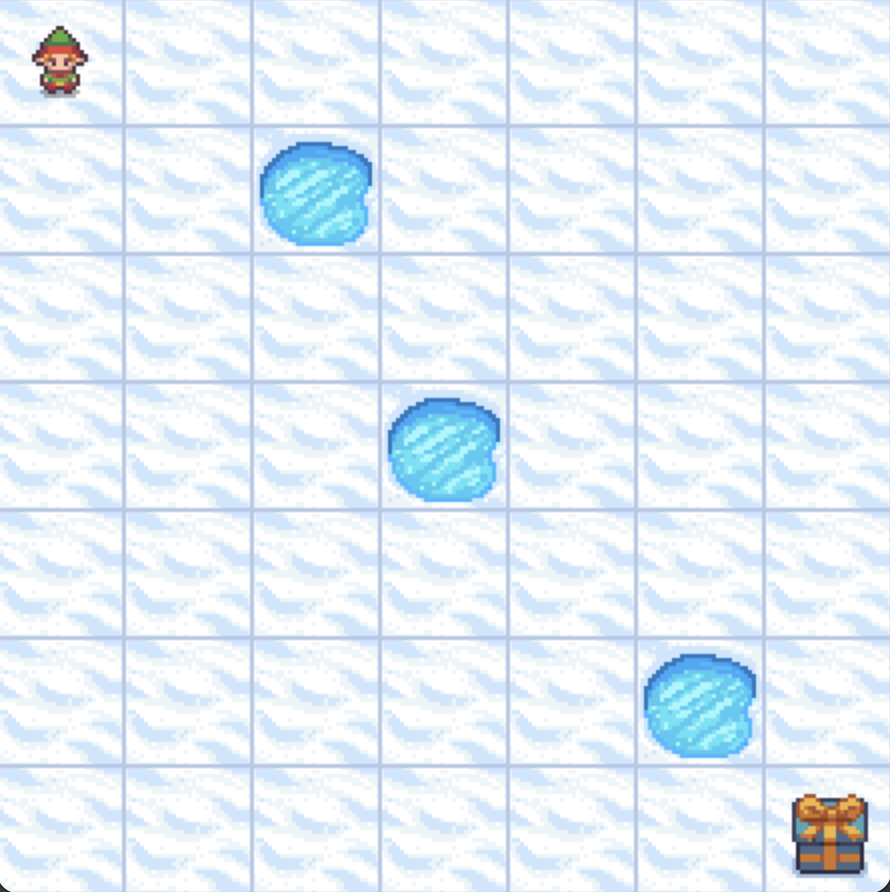
\includegraphics[width=0.8\linewidth]{Env_1.png}
        \caption{Carte pour le cas 1}\label{fig:map_11}
    \end{minipage}
    \hfill
    \begin{minipage}{0.32\textwidth}
        \centering
        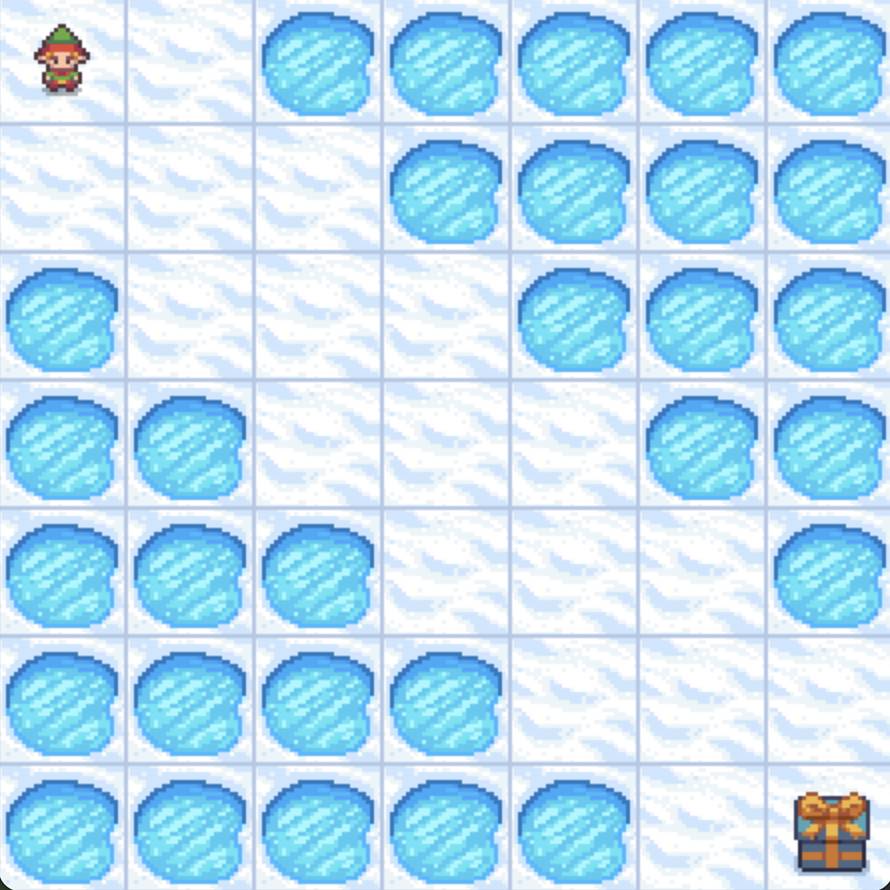
\includegraphics[width=0.8\linewidth]{Env_2.png}
        \caption{Carte pour le cas 2}\label{fig:map_22}
    \end{minipage}
    \hfill
     \begin{minipage}{0.32\textwidth}
        \centering
        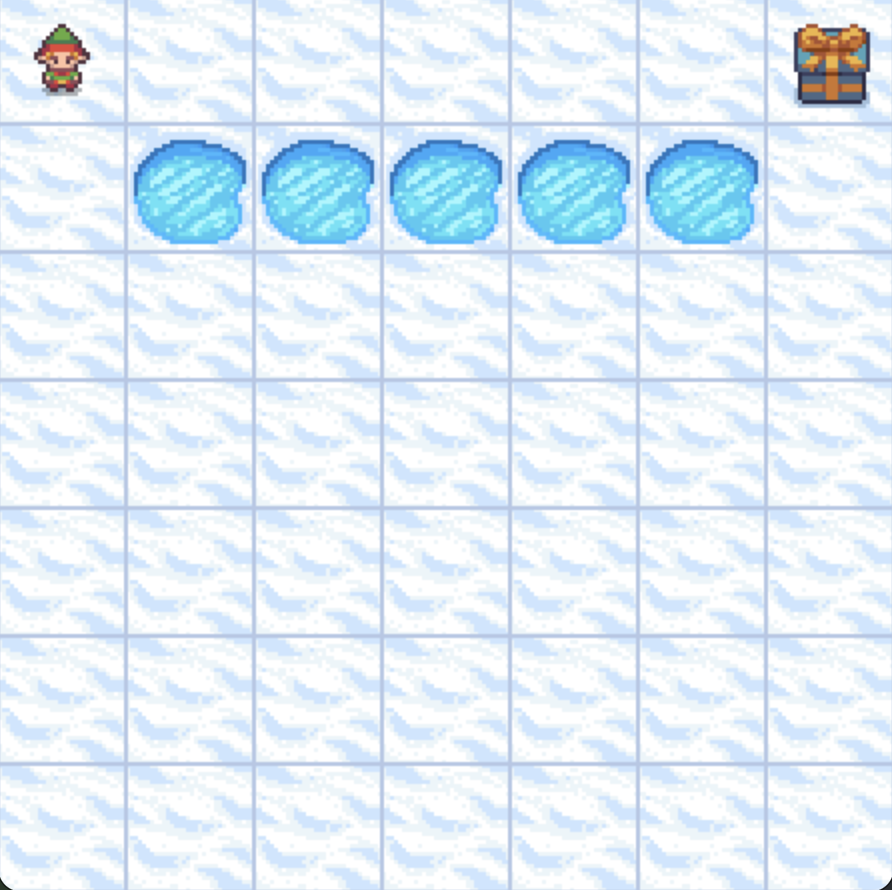
\includegraphics[width=0.8\linewidth]{Env_3.png}
        \caption{Carte pour le cas 3}\label{fig:map_33}
    \end{minipage}
\end{figure}




\section{Stratégies considérées}

Pour résoudre les environnements que nous avons conçus, nous avons sélectionné deux stratégies d'apprentissage par renforcement basées sur les différences temporelles (TD learning) : \textbf{Q-learning} [Watkins, 1989] et \textbf{SARSA} [Rummery et Niranjan, 1994].

\textbf{Motivation du choix :} Ces deux stratégies ont été choisies car elles illustrent deux approches différentes de l'apprentissage de la fonction de valeur : l'apprentissage \textit{off-policy} pour le Q-learning, et \textit{on-policy} pour SARSA. Les comparer est pertinent pour nos cas d'étude (notamment les cas 2 et 3), car elles gèrent le risque de manière très différente face à la stochasticité de l'environnement (glissades possibles).

\subsection{Q-learning (off-policy)}

Le Q-learning vise à apprendre la fonction de valeur d'action optimale $Q^*(s, a)$, indépendamment de la politique suivie par l'agent pour explorer l'environnement. Le fonctionnement est décrit dans le livre de Sutton \& Barto \cite{rlbook}.
%\textbf{Fonctionnement :} À chaque pas de temps, l'agent met à jour la valeur de l'action qu'il vient d'effectuer en supposant que l'action suivante sera la meilleure possible (greedy), même si sa politique d'exploration (par exemple $\epsilon$-greedy) le pousse à faire un choix aléatoire. 
%La règle de mise à jour s'écrit :
%$$Q(S_t, A_t) \leftarrow Q(S_t, A_t) + \alpha \left[ R_{t+1} + \gamma \max_{a} Q(S_{t+1}, a) - Q(S_t, A_t) \right]$$

Le Q-learning a donc tendance à ignorer les risques inhérents à l'exploration lors de sa planification, ce qui le pousse à trouver le chemin absolu le plus court ou le plus rentable, au risque de subir davantage de chutes pendant l'apprentissage.

\subsection{SARSA (on-policy)}

SARSA (State-Action-Reward-State-Action) apprend la fonction de valeur d'action $Q^\pi(s, a)$ associée à la politique $\pi$ que l'agent est en train d'exécuter. Le fonctionnement est décrit dans le livre de Sutton \& Barto \cite{rlbook}.

%\textbf{Fonctionnement :} Contrairement au Q-learning, la mise à jour de SARSA utilise l'action $A_{t+1}$ qui a été réellement sélectionnée par la politique d'exploration pour l'état suivant.
%:
%$$Q(S_t, A_t) \leftarrow Q(S_t, A_t) + \alpha \left[ R_{t+1} + \gamma Q(S_{t+1}, A_{t+1}) - Q(S_t, A_t) \right]$$

Puisque SARSA tient compte des actions d'exploration (qui peuvent être sous-optimales ou dangereuses), l'algorithme a conscience du danger. Dans un environnement pénalisant et glissant, SARSA convergera vers un chemin souvent plus long, mais beaucoup plus sûr (loin des trous).

\section{Méthodologie expérimentale}

Afin de quantifier l'atteinte des objectifs de notre étude et de garantir la reproductibilité de nos résultats, nous avons mis en place le protocole expérimental détaillé ci-dessous.

\subsection{Implémentation et configuration}

Étant donné que le Q-learning et SARSA sont des méthodes tabulaires (l'espace d'états et d'actions étant discret et de petite taille), nous n'utilisons pas de librairies de Deep RL. Les environnements sont générés et gérés via la librairie \textbf{Gymnasium}, tandis que les algorithmes, les politiques d'exploration et les tables $Q$ sont implémentés mathématiquement à l'aide de \textbf{NumPy}.

La configuration de la stratégie d'exploration repose sur une politique $\epsilon$-greedy. Pour les deux algorithmes, les hyperparamètres sont configurés de manière identique pour permettre une comparaison équitable :
\begin{itemize}
    \item \textbf{Taux d'apprentissage ($\alpha$)} : Fixé à 0.1 pour assurer une mise à jour stable des valeurs $Q$.
    \item \textbf{Facteur d'escompte ($\gamma$)} : Fixé à 0.99 pour donner une forte importance aux récompenses futures.
    \item \textbf{Taux d'exploration ($\epsilon$)} : Initialisé à 1.0 (exploration totale), avec une décroissance exponentielle jusqu'à une valeur minimale de 0.01 pour converger vers l'exploitation.
\end{itemize}

\subsection{Paramètres expérimentaux}

Pour assurer la validité statistique de l'étude, les expériences respectent les paramètres de reproductibilité suivants :
\begin{itemize}[noitemsep, topsep=0pt]
    \item \textbf{Pas de temps d'apprentissage :} Chaque algorithme s'entraîne sur un total de \textbf{100 000 pas de temps (\textit{timesteps})} par cas d'étude. Cela garantit une convergence correcte des tables de valeurs, comme le montre la Figure 4.
    \item \textbf{Durée des épisodes :} La longueur maximale d'un épisode est bornée à \textbf{100 pas} (limite standard de \textit{FrozenLake}). Si l'agent n'a pas atteint l'objectif ou n'est pas tombé dans un trou au bout de 100 pas, l'épisode est arrété pour éviter les boucles infinies.
    \item \textbf{Nombre de répétitions :} Afin de lisser la variance induite par l'exploration et les glissades stochastiques, chaque expérience est répétée sur 5 graines aléatoires (\textit{seeds}) différentes.
\end{itemize}

\subsection{Indicateurs de performance}

Pour évaluer la capacité des stratégies à résoudre les défis spécifiques de nos trois cartes (efficacité, évitement, compromis), nous utilisons les indicateurs de performance suivants :
\begin{enumerate}[noitemsep, topsep=0pt]
    \item \textbf{La récompense cumulative moyenne (\textit{Reward}) :} L'indicateur de base, combinant les gains liés à l'objectif et les pénalités environnementales (trous, temps).
    \item \textbf{Le taux de chute (\textit{Fall Rate}) :} Le pourcentage d'épisodes se terminant sur une tuile fatale (H). Ce critère est indispensable pour quantifier la prudence de SARSA par rapport au Q-learning, en particulier dans les cas 2 et 3.
    \item \textbf{Le taux de succès (\textit{Success rate}) :} Proportion d'épisodes où l'agent a atteint le cadeau, reflétant la qualité de la politique apprise en fin d'entraînement.
\end{enumerate}

% lancé avec  python experiment.py depuis ./RL-FrozenLake
\section{Résultats}

Pour le cas 1, les deux stratégies obtiennent de très bonnes performances. Les écarts entre Q-Learning et SARSA restent faibles, ce qui montre qu’elles apprennent toutes deux une politique efficace dans un environnement peu risqué.

Dans le cas 2, les performances baissent pour les deux méthodes, ce qui confirme que ce scénario est plus difficile. SARSA obtient un taux de succès légèrement supérieur, mais aussi davantage de chutes, tandis que les récompenses moyennes restent très proches. Cela peut s’expliquer par la différence de mise à jour entre les deux méthodes.

Le cas 3 est celui où la différence est la plus nette. Q-Learning y obtient une meilleure récompense moyenne, un meilleur taux de succès et moins de chutes que SARSA. Dans ce type de scénario, Q-Learning peut être meilleur car il préfère les trajectoires qui semblent optimales, alors que SARSA apprendra celle qui la pénalise le moins pendant l'entrainement.

%Analyse :

%Sarsa prends moins de risque car il choisi vraiment la politique pendant l'entrainement, donc dans le couloir il est prudent et fait mieux, mais dans le double choix de passage, sa prudence fait qu'il est moins optimal que Q-learning qui prends ce qui est le mieux cyniquement, car il n'en paye pas les consequences

% V2 Pour le cas testant l'efficacité, on retrouve ce que l'on attendait c'est-à-dire que les deux stratégies performent toutes les deux.

%En revanche, on observe que SARSA est plus performant (en terme de récompense moyenne) sur le Cas 2 grâce à sa prise de risque minimisée. Contrairement au Q-learning, qui prend plus de risque car il ne paye pas immédiamment la conséquence de ses choix.

%Pour le cas 3, le Q-Learning apporte de meilleurs résultats pour les mêmes raisons, en n'étant pas punit directement lors de son entraînement, l'agent ne "perçoit" pas le danger que représente le plus court chemin. Même si étonnamment, l'agent SARSA tombe plus souvent dans des trous que Q-Learning.

% Cas 1 : efficacité
% Cas 2 : evitement
% Cas 3 : compromis
\begin{table}[ht]
\centering
\begin{tabular}{llccc}
\toprule
\textbf{Cas d'étude} & \textbf{Stratégie} & \textbf{Récompense moyenne} & \textbf{Taux de chute} & \textbf{Taux de succès} \\
\midrule

\multirow{2}{*}{Cas 1: Efficacité}
  & Q-Learning & 0.7678 & 4.0\% & 95.8\% \\
  & SARSA      & 0.7877 & 5.5\% & 94.5\% \\
\midrule

\multirow{2}{*}{Cas 2 : Évitement}
  & Q-Learning & 0.4180 & 15.6\% & 57.4\% \\
  & SARSA      & 0.4194 & 18.6\% & 60.5\% \\
\midrule

\multirow{2}{*}{Cas 3: Compromis}
  & Q-Learning & 0.2056 & 17.3\% & 82.5\% \\
  & SARSA      & 0.0604 & 23.1\% & 76.8\% \\
  
\bottomrule
\end{tabular}
\vspace{0.2em}
\caption{Comparaison des performances des stratégies considérées}
\label{tab:comparaison}
\end{table}

\begin{figure}[H]
    \centering
    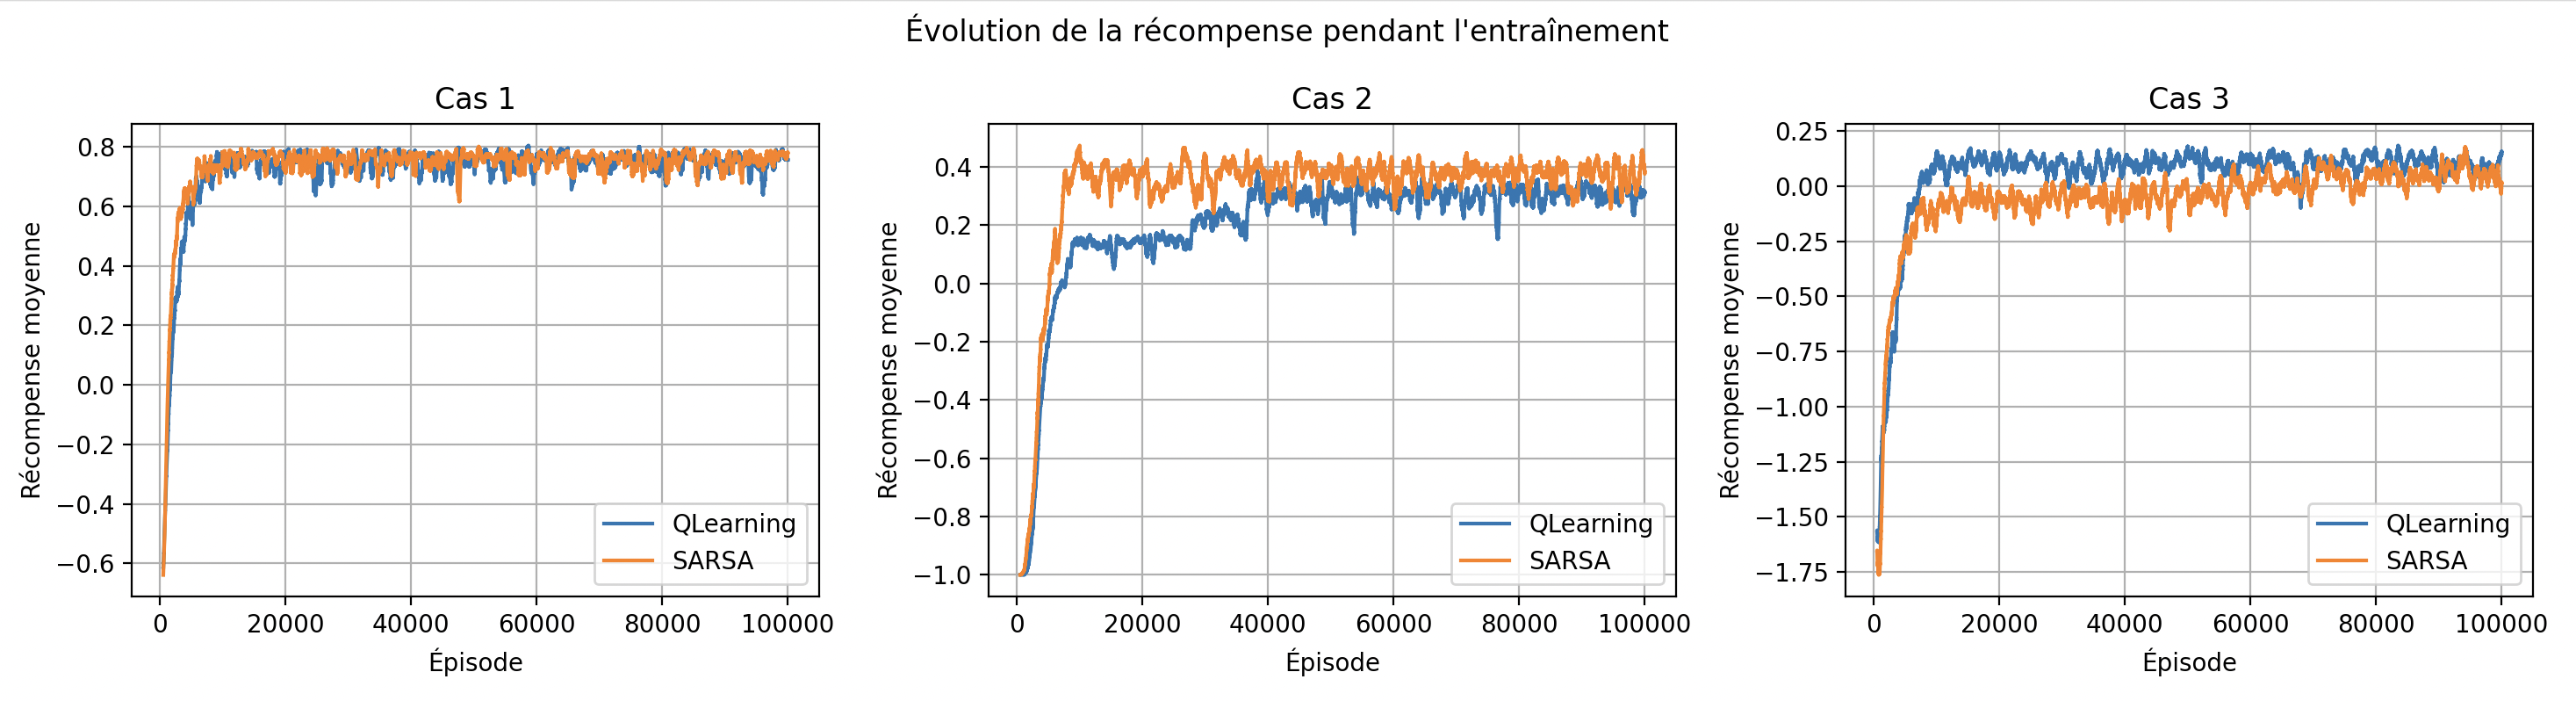
\includegraphics[width=1\linewidth]{Entrainement.png}
    \caption{Visualisation de l'entraînement des stratégies pour tous les environements}
    \label{fig:training}
\end{figure}


% BILBIOGRAPHY --------------------------
\newpage
\begin{thebibliography}{99}

    \bibitem{rlbook}
    Sutton, Richard S. and Barto, Andrew G.
	\newblock Reinforcement learning: an introduction
	\newblock University of Cambridge, 2018

    \bibitem[Watkins(1989)]{watkins1989qlearning}
    Christopher J. C. H. Watkins.
    \newblock Learning from delayed rewards.
    \newblock PhD thesis, University of Cambridge, 1989.
    
    \bibitem[Rummery and Niranjan(1994)]{rummery1994sarsa}
    Gavin A. Rummery and Mahesan Niranjan.
    \newblock On-line Q-learning using connectionist systems.
    \newblock Technical Report CUED/F-INFENG/TR 166, University of Cambridge, 1994.

    \bibitem[Harris et al.(2020)]{numpy}
    Charles R. Harris et al.
    \newblock Array programming with NumPy.
    \newblock Nature, 585:357-362, 2020.

    \bibitem[Farama Foundation(2023)]{gymnasium}
    Farama Foundation.
    \newblock Gymnasium: A standard API for reinforcement learning environments.
    \newblock \url{https://gymnasium.farama.org}, 2023.
    
\end{thebibliography}

\end{document}

% 1.5 et 100_00 pour cas 3 
Learning : recompense moyenne:  0.7484, chutes: 7.5%, succès: 93.0%
SARSA : recompense moyenne:  0.7848, chutes: 7.1%, succès: 94.4%

Cas 2
QLearning : recompense moyenne:  0.3400, chutes: 21.3%, succès: 53.0%
SARSA : recompense moyenne:  0.3820, chutes: 28.1%, succès: 65.0%

Cas 3
QLearning : recompense moyenne: -0.1328, chutes: 26.7%, succès: 74.4%
SARSA : recompense moyenne: -0.0972, chutes: 41.4%, succès: 74.8%

% 1.75 
Cas 1
QLearning : recompense moyenne:  0.7484, chutes: 7.5%, succès: 93.0%
SARSA : recompense moyenne:  0.7848, chutes: 7.1%, succès: 94.4%

Cas 2
QLearning : recompense moyenne:  0.3400, chutes: 21.3%, succès: 53.0%
SARSA : recompense moyenne:  0.3820, chutes: 28.1%, succès: 65.0%

Cas 3
QLearning : recompense moyenne:  0.1906, chutes: 24.4%, succès: 80.2%
SARSA : recompense moyenne:  0.1028, chutes: 44.2%, succès: 74.4%


\multirow{2}{*}{Cas 1: Efficacité }
  & Q-Learning & 0.7484 & 7.5\% & 93.0\% \\
  & SARSA      & 0.7848 & 7.1\% & 94.4\% \\
\midrule

\multirow{2}{*}{Cas 2 : Évitement}
  & Q-Learning & 0.3400 & 31.3\% & 53.0\% \\
  & SARSA      & 0.3820 & 28.1\% & 65.0\% \\

\midrule

\multirow{2}{*}{Cas 3: Compromis}
  & Q-Learning & 0.1906 & 24.4\% & 80.2\% \\
  & SARSA      & 0.1028 & 44.2\% & 74.4\% \\